\chapter{Protein-GAG binding site prediction via electrostatic potential analysis}

In this chapter we present a simple and yet efficient method for predicting
where on a protein a GAG would most likely bind, suggesting which amino acid
residues are likely to be involved and which are not. The method is based on
numerical simulation of the electrostatic (i.e.\ Coulomb) potential of a certain
protein in water solution, and manual evaluation of the topology of the Coulomb
potential in space. Subsequently, we apply that method to IL-10 and report our
findings.

\section{Motivation}

Classical molecular docking approaches are used for creating binding predictions
for a given receptor-ligand system. Primarily, the correctness of a prediction
depends on the quality of the underlying physical or phenomenological model, and
whether the system under investigation is within the scope of validity of the
model. Since most molecular docking methods are trained for analyzing a limited
Cartesian volume in a \textit{local} search, application to larger search spaces
dramatically lowers the confidence in the resulting prediction. As a result,
common molecular docking methods should be applied locally, and therefore
require \textit{a priori} knowledge about where on the receptor the ligand most
likely binds. The decision where to center the local search on should be based
on reliable data, otherwise the docking study might be pointless. In the best
case, knowledge about the binding site (the region on the receptor that the
ligand binds to) comes from experimental data, e.g.\ from mutagenesis or NMR
studies.

In other cases, no experimental data is available that provides clues about the
binding site, as is the case with the IL-10-GAG system. In such cases, it makes
sense to consider \textit{in silico} methods for binding site prediction.  With
respect to protein-GAG systems, there is only few published work on this topic.
In \cite{hp_binding_sites_mulloy_2006}, the authors used AutoDock version 2.4
\cite{autodock24} for globally docking rigid heparin molecules to antithrombin
and FGF-2, and found that their docking procedure gave good agreement with the
corresponding crystal structures regarding the overall position of the heparin
binding sites. The authors state that the method may be used as
\enquote{hypothesis generation tool} rather than for providing \enquote{details
of interactions between specific atoms}. In another work
\cite{gandhi_bmp_heparin_binding_sites_2012}, the authors used PatchDock
\cite{patchdock_2002} for globally docking rigid heparin oligosaccharides to
BMP-2 and BMP-14 and state that \enquote{while there has been no validation
of the accuracy of the PatchDock scoring function for heparin interactions,
these docking results suggest the presence of two GAG binding sites in BMP-2}.


None of the authors provides arguments why the docking method of choice should
be valid for protein-GAG systems.



 In that case,
the docking study might be able to provide insights about the receptor- ligand
interaction on an atomic level, i.e.\ with higher resolution than the



 and
also on the sampling performance of the method. We can safely conclude that with
increasing search space, the validity of any prediction

The larger the cartesian search space, the

The validity of binding predictions from classical molecular docking approaches
increases with

Molecular docking approaches

No estimation whether that model is trustable or not

\section{Method}

\subsection{Coulomb potential simulation}

\subsection{Coulomb potential evaluation}

\section{Application to reference systems}

\subsection{Results and discussion}

\section{Application to IL-10}





\begin{figure}
\centering
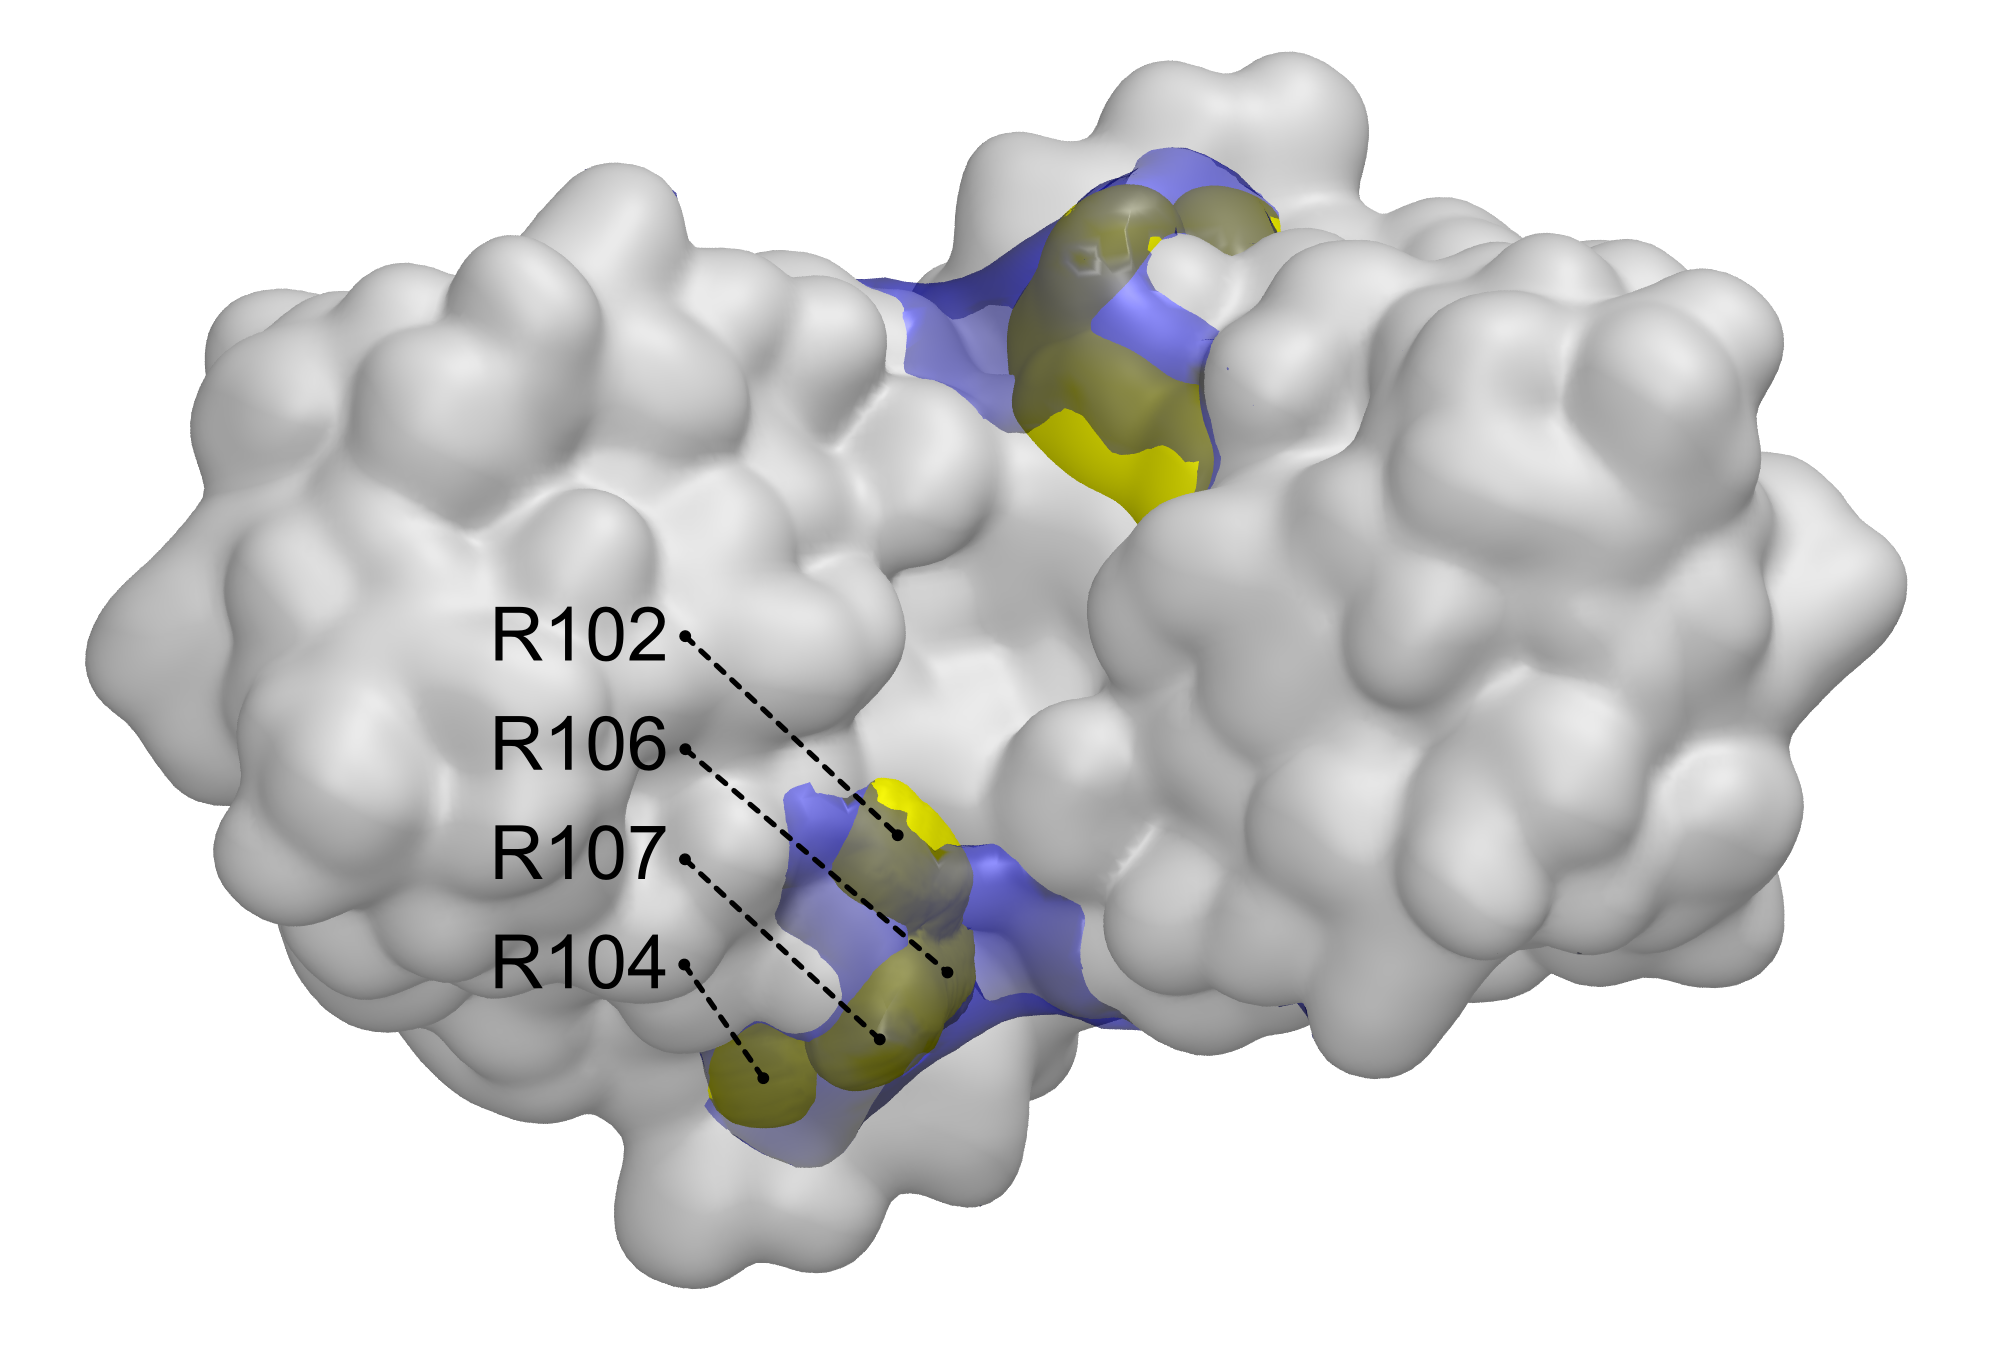
\includegraphics[width=0.9\textwidth]{gfx/bspred/SI_figure_IL-10_coulomb_isosurface_1_9kcalmol.png}
\caption[]{

Isosurface representation of IL-10's Coulomb potential with the isovalue $\Phi =
\SI{1.9}{\kilo\calory\per\mole\per\elementarycharge}$ (blue). The molecular
surface of the IL-10 dimer is shown in gray, the molecular surface of arginines
102, 104, 106, 107 is shown in yellow (structure taken from PDB ID 2ILK). This
representation allows to see where the Coulomb potential (for a given isovalue)
protrudes into space further than the molecular surface, and has been shown to
provide useful evidence about where GAGs bind to a protein \hl{(REF)}. Hence,
IL-10-GAG interaction most likely takes place within the two symmetrically
arranged regions indicated here.

}
\label{fig:bspred:il10_estatic_pred}
\end{figure}




\subsubsection{Electrostatic potential analysis in protein-GAG systems}

\hl{Generalize this section, keep details for DMD chapter. At the moment most of
this is simply copied from the DMD manuscript.}

The electrostatic potential often dominates protein-GAG interaction
\cite{gandhi_structure_2008}. In this section, we discuss the electrostatic
properties of the receptors in the TDS with the goal to determine how these
properties could assist defining a receptor target region for DMD and also to be
able to relate docking performance to electrostatic characteristics of the
receptor.


Poisson-Boltzmann-based numeric calculations of the electrostatic potential of
molecules are most error-prone near the dielectric boundary, i.e.\ on the
molecular surface. We therefore did not simply map the potential on the
molecular surface but analyzed the topology of the potential with an isosurface
representation while varying the isosurface value. This allows for an
understanding  of the distribution of the potential in space and how strongly it
would affect a ligand. \cref{fig:bspred:sdf1_estatic} shows an isosurface of the
Coulomb potential of SDF-1. \cref{fig:bspred:various_estatic} shows analogous
isosurface representations of the electrostatic potential for the other TDS
complexes. For this type of visualization, the isovalue selection was done
individually for each receptor in the TDS such that only a small part of the
isosurface is protruding into space further than the molecular surface of the
receptor.



\begin{figure}
\centering
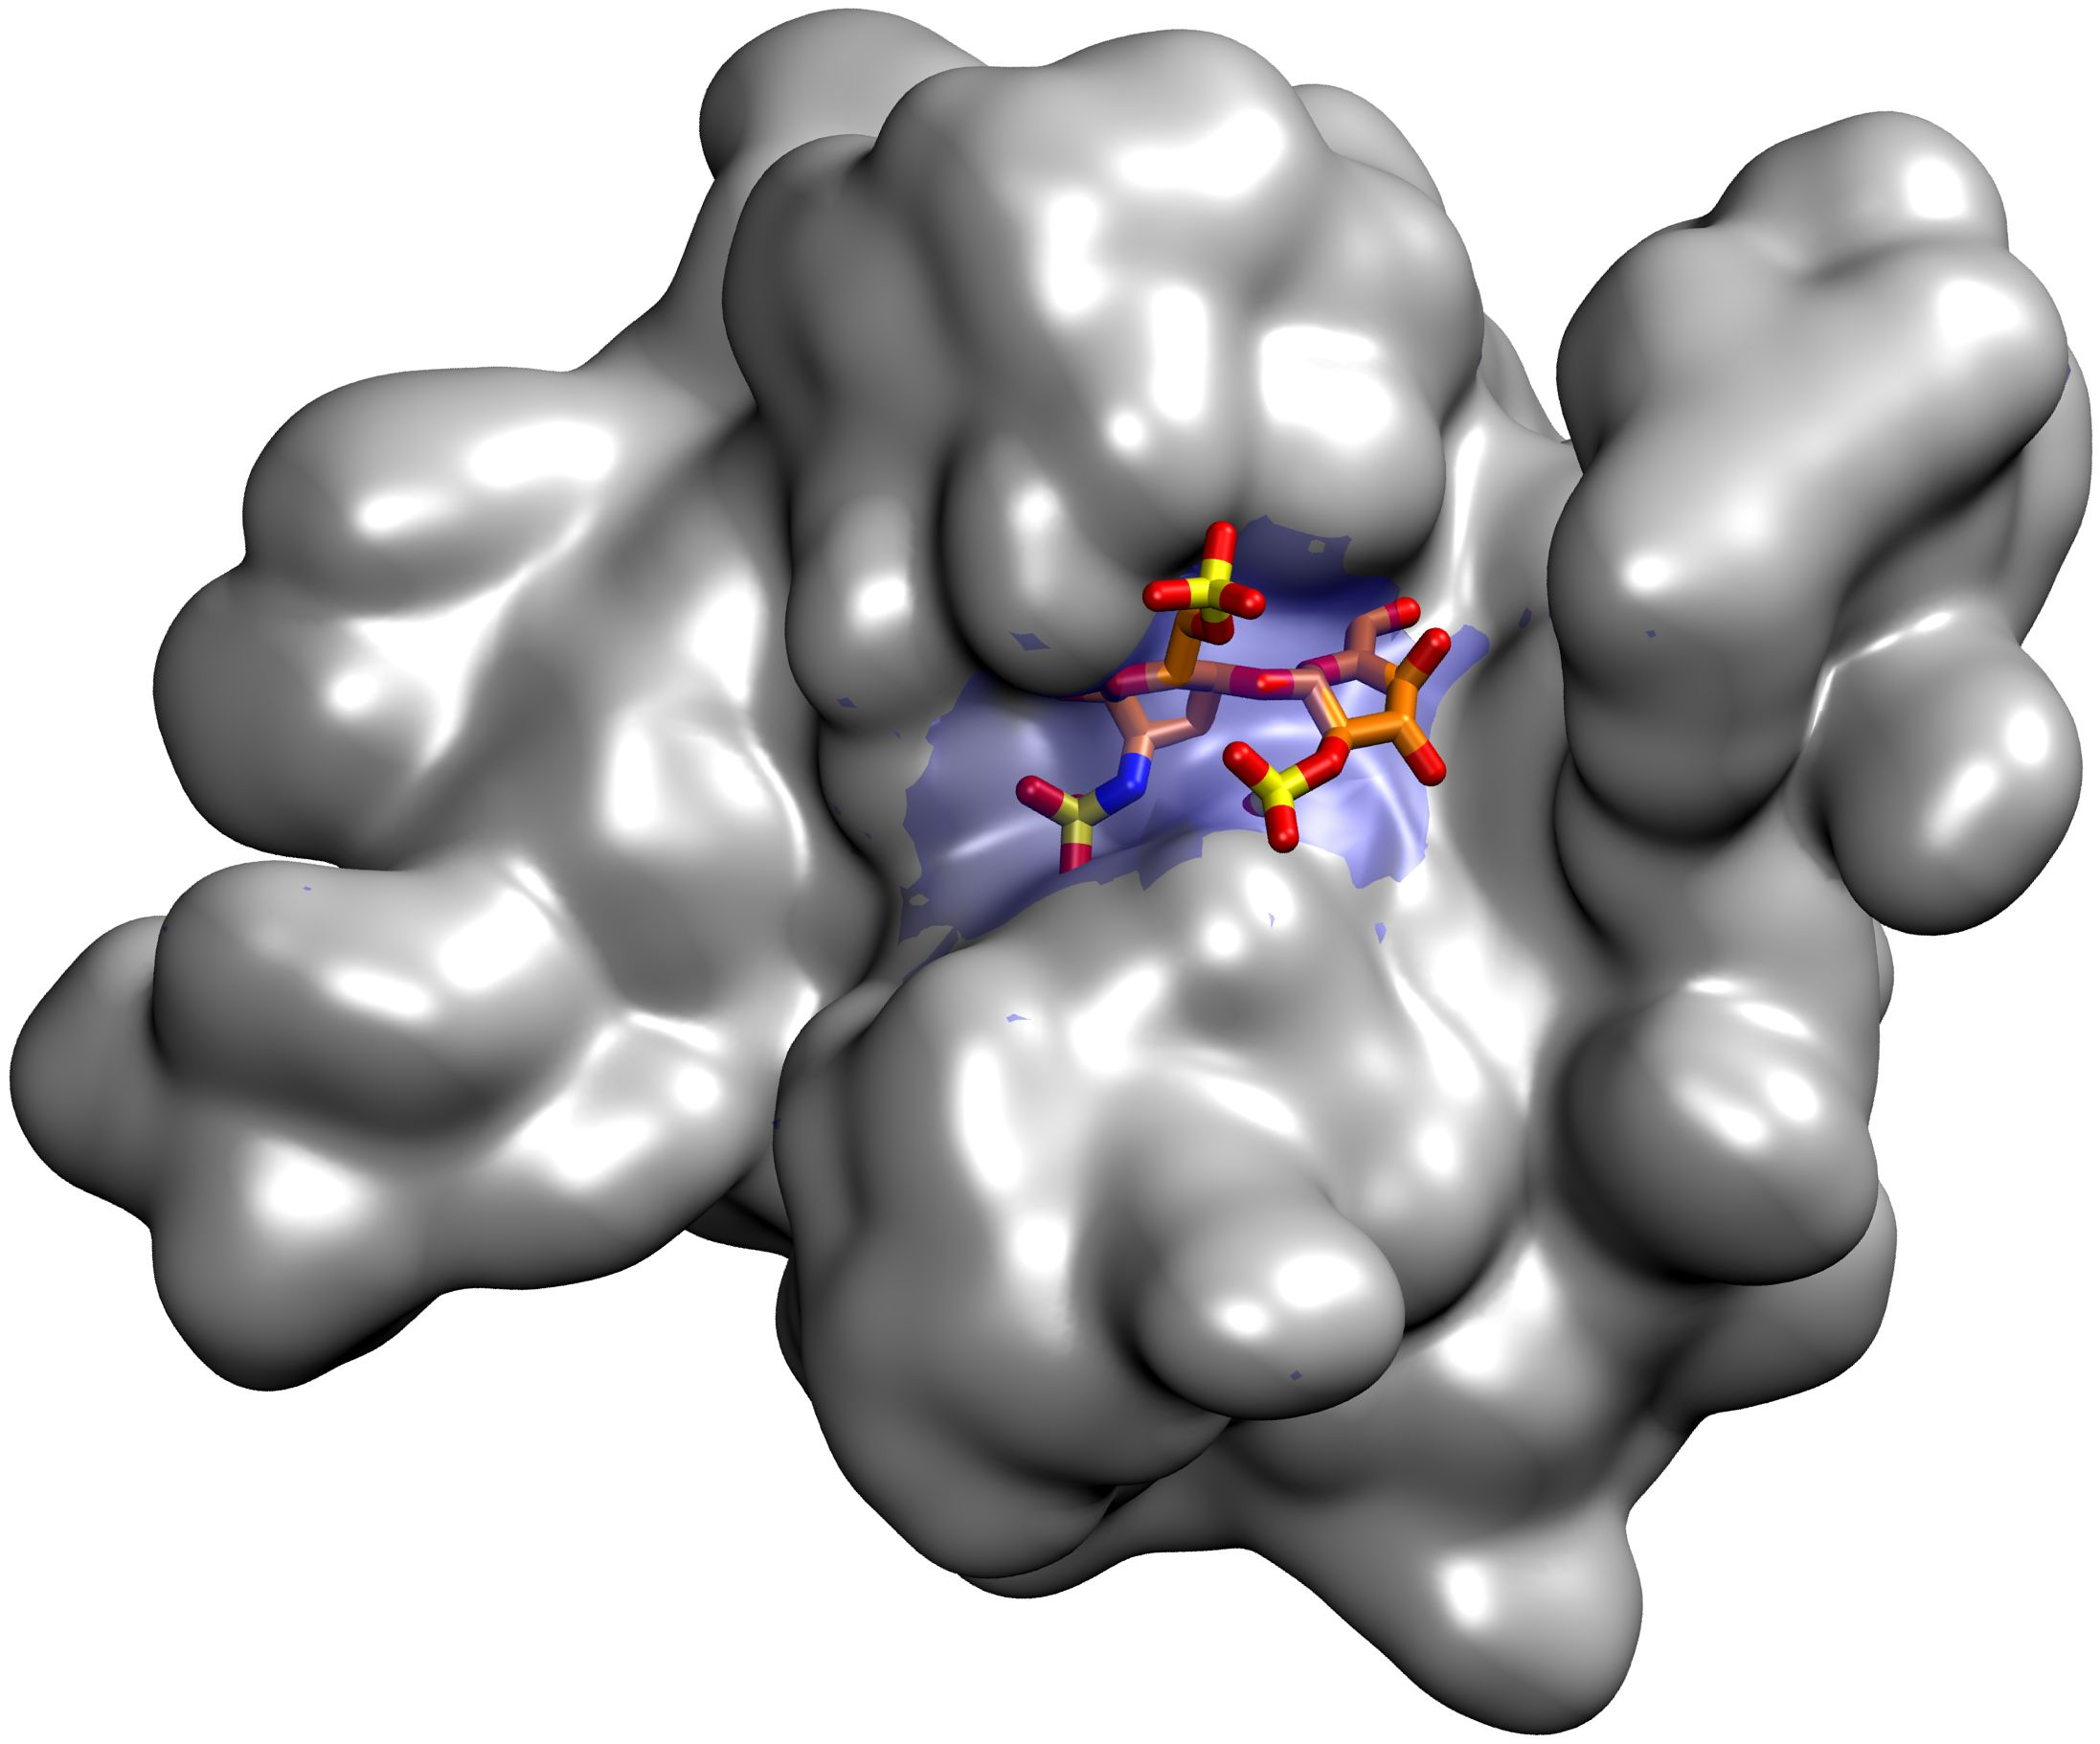
\includegraphics[width=0.9\textwidth]{gfx/bspred/sdf1_isopot_8_5_view1_rotated_jcc_pub_001.jpg}
\caption[]{
Isosurface representation of SDF-1's electrostatic potential with the isovalue
$\Phi = 8.5\,\mathrm{kcal\,mol^{-1}\,e^{-1}}$ (blue). The molecular surface of
the SDF-1 dimer is shown in grey, the heparin ligand as determined
experimentally (PDB ID 2NWG) is shown as sticks with C atoms in orange.
}
\label{fig:bspred:sdf1_estatic}
\end{figure}

Regarding the SDF-1-HP complex, our electrostatic potential evaluation procedure
unambiguously identifies the GAG binding site as determined experimentally. With
$8.5\,\mathrm{kcal\,mol^{-1}\,e^{-1}}$, the isovalue chosen is the largest among
the TDS complexes, indicating that SDF-1 has the strongest electrostatic
attraction to its ligand. In case of FGF2-HP (\cref{fig:bspred:various_estatic}), the
binding site is also unambiguously defined by the electrostatic potential. For
CD44-HA, the net electrostatic interaction between both molecules is slightly
repulsive. There is no obvious relation between the electrostatic properties of
the receptor and the binding site location. CathK and CathKmut exhibit
electrostatic attraction for negatively charged molecules in the experimentally
observed ligand binding site as well as in an adjacent region. We observe that
electrostatic potential analysis provides a clear idea whether GAG-binding to a
given receptor is mainly driven by Coulomb interaction. If a protein is known to
bind GAGs, and the electrostatic potential topology is as unambiguous as in case
of SDF-1 or FGF2, a GAG binding site prediction based on the presented procedure
is reliable. Visualization of the electrostatic potential can also be helpful to
\textit{a priori} exclude regions of the receptor surface when repulsive to
negatively charged ligands. Furthermore, this analysis shows that knowledge
about the electrostatic potential distribution in space can be used to choose a
reasonable ligand \enquote{entry lane} orientation for the tMD pulling process.


\begin{figure}
\centering
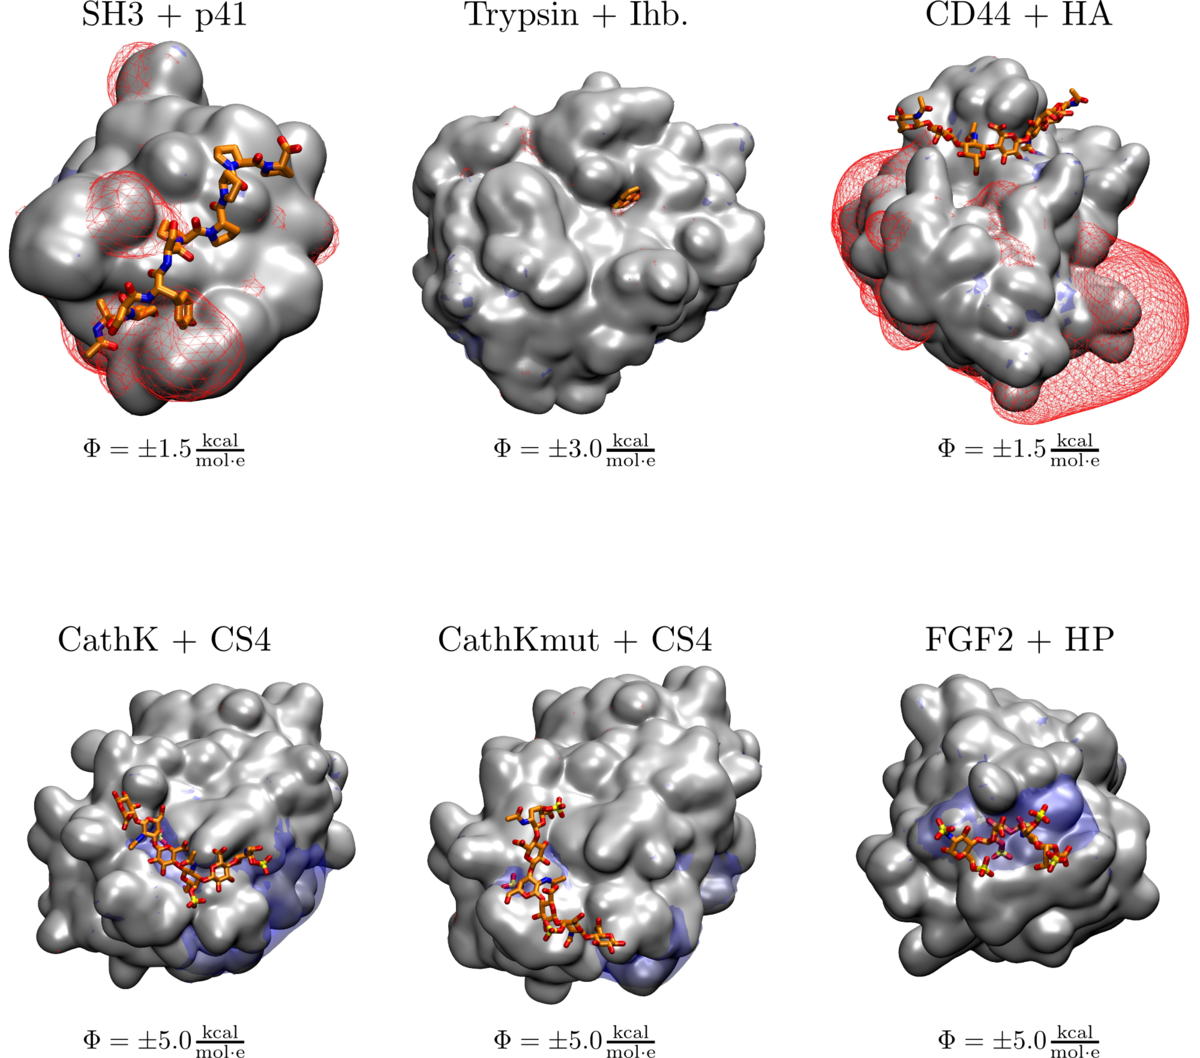
\includegraphics[width=0.9\textwidth]{gfx/bspred/suppl_figure_estatic_distributions_004_1200.png}
\caption[]{
Visualization of the electrostatic potential of the receptors from the TDS
(molecular surfaces in gray) with their ligands as experimentally determined
(shown as sticks with C atoms in orange). Blue/red: Isosurface representation of
the receptor's electrostatic potential with isovalue Ф (attractive/repulsive for
negatively charged molecules, respectively).
}
\label{fig:bspred:various_estatic}
\end{figure}


\hl{Create more convincing Figure than bspred:variousestatic.
Include more interesting complexes, remove uninteresting ones.}

The SH3-p41 complex is dominated by non-polar interactions, rendering the
Coulomb potential analysis inconclusive. Recognition of the Trypsin inhibitor in
its  binding pocket is affected by polar interactions. The electrostatic
potential, however, does not display clear characteristics to predict a binding
region.


